% Created 2020-04-24 vie 10:35
% Intended LaTeX compiler: pdflatex
\documentclass[presentation,aspectratio=1610]{beamer}
\usepackage[utf8]{inputenc}
\usepackage[T1]{fontenc}
\usepackage{graphicx}
\usepackage{grffile}
\usepackage{longtable}
\usepackage{wrapfig}
\usepackage{rotating}
\usepackage[normalem]{ulem}
\usepackage{amsmath}
\usepackage{textcomp}
\usepackage{amssymb}
\usepackage{capt-of}
\usepackage{hyperref}
\usepackage{khpreamble}
\usepackage{pgfplots}
\usepackage{pdfpages}
\usepackage{circuitikz}
\usepgfplotslibrary{groupplots}
\usetikzlibrary{positioning}
\renewcommand*{\not}[1]{\ensuremath{\bar{#1}}}
\renewcommand*{\not}[1]{\ensuremath{\overline{#1}}}
\usetheme{default}
\author{Kjartan Halvorsen}
\date{\today}
\title{Logic control and boolean algebra}
\hypersetup{
 pdfauthor={Kjartan Halvorsen},
 pdftitle={Logic control and boolean algebra},
 pdfkeywords={},
 pdfsubject={},
 pdfcreator={Emacs 26.3 (Org mode 9.3.6)}, 
 pdflang={English}}
\begin{document}

\maketitle

\section{Intro}
\label{sec:org67c67af}



\section{Logic control and boolean algebra}
\label{sec:org81ff278}
\begin{frame}[label={sec:orgc2fb03f}]{A logic control loop}
\begin{center}
\includegraphics[width=\linewidth]{../../figures/logic-control-loop}
\end{center}
\end{frame}

\begin{frame}[label={sec:org895be34}]{Cheese pressing example}
\begin{center}
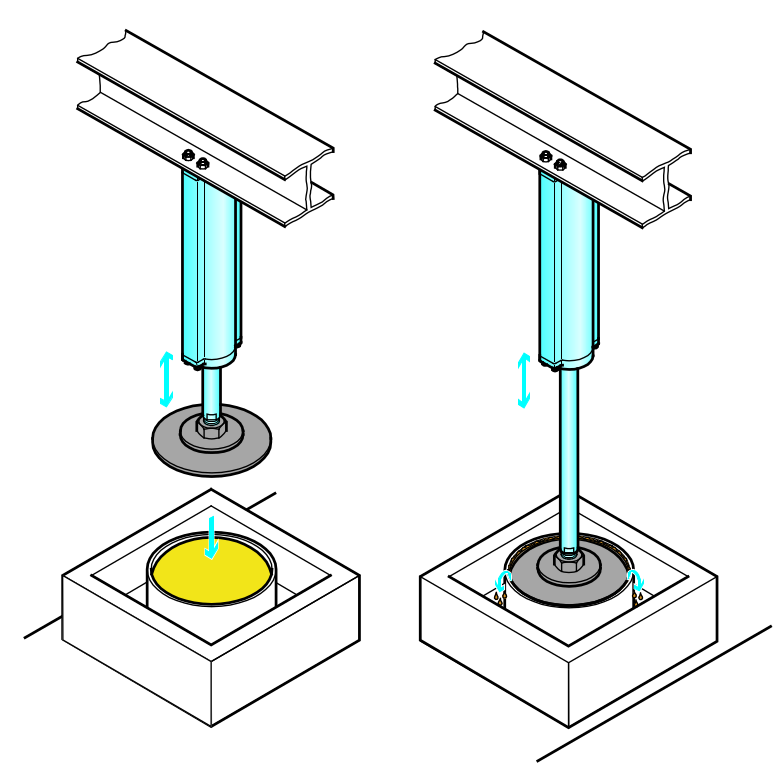
\includegraphics[width=0.5\linewidth]{../../figures/cheese-stamping.png}
\end{center}
\begin{LaTeX}
\{\tiny From FESTO Didactic\}
\end{LaTeX}
\end{frame}

\begin{frame}[label={sec:org3956e0f}]{Cheese pressing example - Variables}
Activating solenoid S1 extends the cylinder, activating solenoid S2 retracts the cylinder.
\begin{columns}
\begin{column}{0.5\columnwidth}
\begin{block}{State variable}
\[ x_k = \begin{cases} 0 & \text{Cylinder retracted}\\1 & \text{Cylinder extended}\end{cases}\]
\end{block}
\begin{block}{Control signal}
\[ u = \begin{bmatrix} u_1\\u_2 \end{bmatrix}, \]
with
\begin{align*}
u_1 &= \begin{cases} 0 & \text{Don't activate S1}\\1 & \text{Activate S1 }\end{cases}\\
u_2 &= \begin{cases} 0 & \text{Don't activate S2}\\1 & \text{Activate S2}\end{cases}\\
\end{align*}
\end{block}
\end{column}

\begin{column}{0.5\columnwidth}
\begin{block}{Command signal}
\[ u_{c} = \begin{cases} 0 & \text{Button unpushed}\\1 & \text{Button pushed}\end{cases}. \]
\end{block}
\end{column}
\end{columns}
\end{frame}

\begin{frame}[label={sec:org08ed2a4}]{Cheese pressing example - Plant dynamics and control law}
Activating solenoid S1 extends the cylinder, activating solenoid S2 retracts the cylinder.
\begin{columns}
\begin{column}{0.5\columnwidth}
\begin{block}{Plant dynamics}
\begin{center}
\begin{tabular}{|cc|cc|}
\hline
 &  & state & \\
\(u_{1,k}\) & \(u_{2,k}\) & \(x_k\) & \(x_{k+1}\)\\
\hline
0 & 0 & 0 & 0\\
0 & 1 & 0 & 0\\
1 & 0 & 0 & 1\\
(1) & (1) & 0 & undefined\\
0 & 0 & 1 & 1\\
0 & 1 & 1 & 0\\
1 & 0 & 1 & 1\\
(1) & (1) & 1 & undefined\\
\hline
\end{tabular}
\end{center}
\end{block}
\end{column}

\begin{column}{0.5\columnwidth}
\begin{block}{Control law}
\begin{center}
\begin{tabular}{|cc|cc|}
\hline
\(x\) & \(u_{c}\) & \(u_1\) & \(u_2\)\\
\hline
0 & 0 & 0 & 0\\
0 & 1 & 1 & 0\\
1 & 0 & 0 & 1\\
1 & 1 & 0 & 1\\
\hline
\end{tabular}
\end{center}
\end{block}
\end{column}
\end{columns}
\end{frame}


\section{Boolean algebra, minterms and maxterms}
\label{sec:org7d592ef}
\begin{frame}[label={sec:orgf5ab4de}]{Boolean algebra}
\(X, Y \in \{0,1\}\)
\begin{columns}
\begin{column}{0.5\columnwidth}
\begin{block}{AND}
\begin{center}
\begin{tabular}{|cc|c|}
\hline
\(X\) & \(Y\) & \(X\) AND \(Y\)\\
\hline
0 & 0 & 0\\
0 & 1 & 0\\
1 & 0 & 0\\
1 & 1 & 1\\
\hline
\end{tabular}
\end{center}

\begin{center}
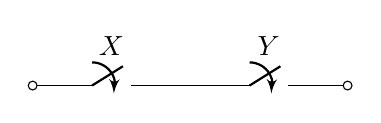
\begin{tikzpicture}
  \draw (0,0) to[switch, label=$X$, o-] (2,0) to[switch, label=$Y$, -o] (4, 0);
\end{tikzpicture}
\end{center}
\alert{Closed circuit \(\Leftrightarrow\) 1}

\alert{Open circuit \(\Leftrightarrow\) 0}
\end{block}
\end{column}

\begin{column}{0.5\columnwidth}
\begin{block}{OR}
\begin{center}
\begin{tabular}{|cc|c|}
\hline
\(X\) & \(Y\) & \(X\) OR \(Y\)\\
\hline
0 & 0 & 0\\
0 & 1 & 1\\
1 & 0 & 1\\
1 & 1 & 1\\
\hline
\end{tabular}
\end{center}

\begin{center}
\begin{tikzpicture}
  \draw (0,0) to[switch, label=$X$, o-o] (4,0);
  \draw (1,0) to[short] (1,-1) to[switch, l_=$Y$, ] (3, -1) to[short] (3, 0);
\end{tikzpicture}
\end{center}
\end{block}
\end{column}
\end{columns}
\end{frame}
\begin{frame}[label={sec:org442a143}]{Boolean algebra, contd}
\(X, Y, Z \in \{0,1\}\)

\begin{center}
\begin{tabular}{r|c|c|}
 & Property & Dual\\
\hline
Properties of 0 and 1 & \(X+0=X\) & \(X\cdot 0=0\)\\
 & \(X+1=1\) & \(X \cdot 1 = X\)\\
Idempotent & \(X+X=X\) & \(X\cdot X = X\)\\
Complementarity & \(X+\not{X}=1\) & \(X\cdot \not{X}=0\)\\
Involution & \(\not{\not{X}}=X\) & \\
Commutative & \(X+Y=Y+X\) & \(X\cdot Y = Y\cdot X\)\\
Associative & \((X+Y) + Z = X + (Y+Z)\) & \((XY)Z = Z(YZ)\)\\
Distributive & \(X\cdot (Y+Z) = XY + XZ\) & \(X+YZ=(X+Y)(X+Z)\)\\
\hline
\end{tabular}
\end{center}
\end{frame}

\begin{frame}[label={sec:org11fe889}]{Boolean algebra, contd}
\(X, Y, Z \in \{0,1\}\)

\begin{center}
\begin{tabular}{r|c|c|}
 & Theorem & Dual\\
\hline
Absorption & \(X+XY=X(1+Y)=X\) & \(X(X+Y)=X\)\\
Logic adjacency & \(XY + X\not{Y} = X(Y+\not{Y}) =X\) & \((X+Y)(X+\not{Y}) = X\)\\
De Morgan's & \(\not{X+Y}=\not{X}\not{Y}\) & \(\not{XY} = \not{X} + \not{Y}\)\\
\hline
\end{tabular}
\end{center}
\end{frame}


\section{Latching circuit}
\label{sec:org21f48c3}
\begin{frame}[label={sec:org1e4f80e}]{An electrical circuit with memory}
\begin{columns}
\begin{column}{0.6\columnwidth}
\begin{block}{Latching circuit}
\begin{LaTeX}
\begin{center}
         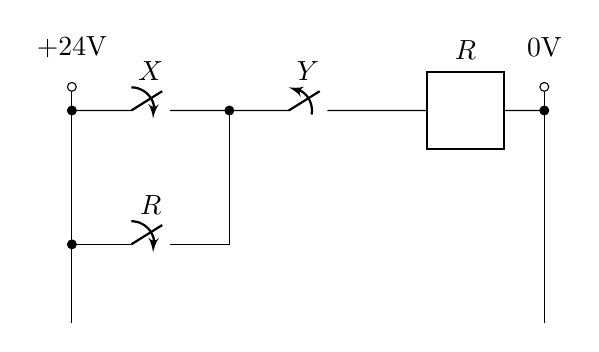
\begin{tikzpicture}
           \node at (0,0.5) {+24V};
           \node at (6,0.5) {0V};
           \draw (0,0) to[short, o-]  (0,-3);
           \draw (6,0) to[short, o-](6,-3);
           \draw (0,-0.3) to[switch, *-, label=$X$] (2,-0.3) to[ opening switch, label=$Y$, ] (4,-0.3) to[short] (4,-0.3) to[twoport, label=$R$, -*] (6,-0.3);
           \draw (0,-2) to[switch, *-, label=$R$] (2,-2)  to[short,-*] (2,-0.3);
         \end{tikzpicture}
\end{center}
\end{LaTeX}
\end{block}
\end{column}

\begin{column}{0.4\columnwidth}
\begin{block}{Truth table}
\begin{center}
\begin{tabular}{|ccc|c|}
\(X\) & \(Y\) & \(R_k\) & \(R_{k+1}\)\\
\hline
0 & 0 & 0 & \\
0 & 0 & 1 & \\
0 & 1 & 0 & \\
0 & 1 & 1 & \\
1 & 0 & 0 & \\
1 & 0 & 1 & \\
1 & 1 & 0 & \\
1 & 1 & 1 & \\
\hline
\end{tabular}
\end{center}
\end{block}
\end{column}
\end{columns}
\end{frame}

\begin{frame}[label={sec:orgfc96bd9}]{An electrical circuit with memory}
\begin{columns}
\begin{column}{0.6\columnwidth}
\begin{block}{Latching circuit}
\begin{LaTeX}
\begin{center}
         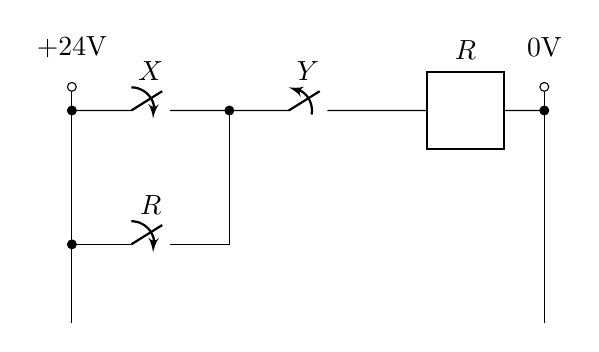
\begin{tikzpicture}
           \node at (0,0.5) {+24V};
           \node at (6,0.5) {0V};
           \draw (0,0) to[short, o-]  (0,-3);
           \draw (6,0) to[short, o-](6,-3);
           \draw (0,-0.3) to[switch, *-, label=$X$] (2,-0.3) to[ opening switch, label=$Y$, ] (4,-0.3) to[short] (4,-0.3) to[twoport, label=$R$, -*] (6,-0.3);
           \draw (0,-2) to[switch, *-, label=$R$] (2,-2)  to[short,-*] (2,-0.3);
         \end{tikzpicture}
\end{center}
\end{LaTeX}
\end{block}
\end{column}

\begin{column}{0.4\columnwidth}
\begin{block}{Truth table}
\begin{center}
\begin{tabular}{|ccc|c|}
\(X\) & \(Y\) & \(R_k\) & \(R_{k+1}\)\\
\hline
0 & 0 & 0 & 0\\
0 & 0 & 1 & 1\\
0 & 1 & 0 & 0\\
0 & 1 & 1 & 0\\
1 & 0 & 0 & 1\\
1 & 0 & 1 & 1\\
1 & 1 & 0 & 0\\
1 & 1 & 1 & 0\\
\hline
\end{tabular}
\end{center}
\end{block}
\end{column}
\end{columns}
\end{frame}

\section{Return to example}
\label{sec:orgc94041b}
\begin{frame}[label={sec:orge36e1ee}]{Cheese pressing example - Plant dynamics and control law revisited}
Activating solenoid S1 extends the cylinder, activating solenoid S2 retracts the cylinder.
\begin{columns}
\begin{column}{0.5\columnwidth}
\begin{block}{Plant dynamics}
\begin{center}
\begin{tabular}{|cc|cc|}
\hline
 &  & state & \\
\(u_{1,k}\) & \(u_{2,k}\) & \(x_k\) & \(x_{k+1}\)\\
\hline
0 & 0 & 0 & 0\\
0 & 1 & 0 & 0\\
1 & 0 & 0 & 1\\
(1) & (1) & 0 & undefined\\
0 & 0 & 1 & 1\\
0 & 1 & 1 & 0\\
1 & 0 & 1 & 1\\
(1) & (1) & 1 & undefined\\
\hline
\end{tabular}
\end{center}

\begin{align*} 
  x_{k+1} &= u_{1,k}\not{u_{2,k}}\not{x_k} + \not{u_{1,k}}\not{u_{2,k}}x_k + u_{1,k}\not{u_{2,k}}x_k\\ &=  \not{u_{1,k}}\not{u_{2,k}}x_k + u_{1,k}\not{u_{2,k}}
\end{align*}
\end{block}
\end{column}

\begin{column}{0.5\columnwidth}
\begin{block}{Control law}
\begin{center}
\begin{tabular}{|cc|cc|}
\hline
\(x\) & \(u_{c}\) & \(u_1\) & \(u_2\)\\
\hline
0 & 0 & 0 & 0\\
0 & 1 & 1 & 0\\
1 & 0 & 0 & 1\\
1 & 1 & 0 & 1\\
\hline
\end{tabular}
\end{center}

\begin{align*}
  u_1 &= \not{x}u_c\\
  u_2 &= x\not{u_c} + xu_c = x
\end{align*}
\end{block}
\end{column}
\end{columns}
\end{frame}



\begin{frame}[label={sec:org4f9c0a5}]{Cheese pressing example - Control law}
\begin{columns}
\begin{column}{0.5\columnwidth}
\begin{block}{Solenoid S1}
\[u_1 = \not{x}u_c \]
\begin{LaTeX}
\begin{center}
  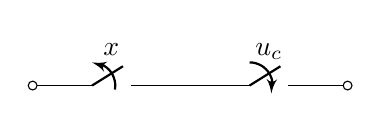
\begin{tikzpicture}
    \draw (0,0) to[opening switch, o-, label=$x$] (2,0) to[ switch, label=$u_c$, -o] (4,0);
  \end{tikzpicture}
\end{center}
\end{LaTeX}
\end{block}
\end{column}

\begin{column}{0.5\columnwidth}
\begin{block}{Solenoid S2}
\[u_2 = x \]
\begin{LaTeX}
\begin{center}
  \begin{tikzpicture}
    \draw (0,0) to[opening switch, o-o, label=$x$] (4,0);
  \end{tikzpicture}
\end{center}
\end{LaTeX}
\end{block}
\end{column}
\end{columns}
\end{frame}


\begin{frame}[label={sec:org099ba24}]{Cheese pressing example - Implementation of the control law}
\begin{LaTeX}
\begin{center}
         \begin{tikzpicture}
           \node at (0,0.5) {+24V};
           \node at (10,0.5) {0V};
           \draw (0,0) to[short, o-]  (0,-5);
           \draw (10,0) to[short, o-](10,-5);
         \end{tikzpicture}
\end{center}
\end{LaTeX}
\end{frame}

\begin{frame}[label={sec:orge976c20}]{Cheese pressing example - Implementation of the control law, solution}
\begin{LaTeX}
\begin{center}
         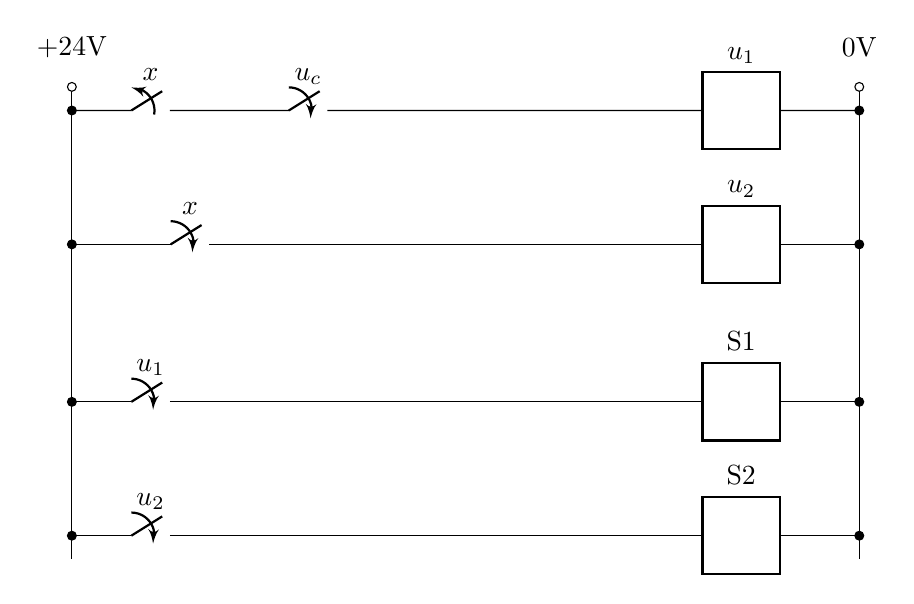
\begin{tikzpicture}
           \node at (0,0.5) {+24V};
           \node at (10,0.5) {0V};
           \draw (0,0) to[short, o-]  (0,-6);
           \draw (10,0) to[short, o-](10,-6);
           \draw (0,-0.3) to[opening switch, *-, label=$x$] (2,-0.3) to[ switch, label=$u_c$, ] (4,-0.3) to[short] (7,-0.3) to[twoport, label=$u_1$, -*] (10,-0.3);
           \draw (0,-2) to[switch, *-, label=$x$] (3,-2)  to[short] (7,-2) to[twoport, label=$u_2$, -*] (10,-2);
           \draw (0,-4) to[switch, *-, label=$u_1$] (2,-4) to[short] (7,-4)  to[twoport, label=S1, -*] (10,-4);
           \draw (0,-5.7) to[switch, *-, label=$u_2$] (2,-5.7)  to[short] (7,-5.7)  to[twoport, label=S2, -*] (10,-5.7);

         \end{tikzpicture}
\end{center}
\end{LaTeX}
\end{frame}

\section{The lab assignment}
\label{sec:orga08f675}
\begin{frame}[label={sec:org4244982}]{Implementing the sequence A+B+B-A-}
\begin{center}
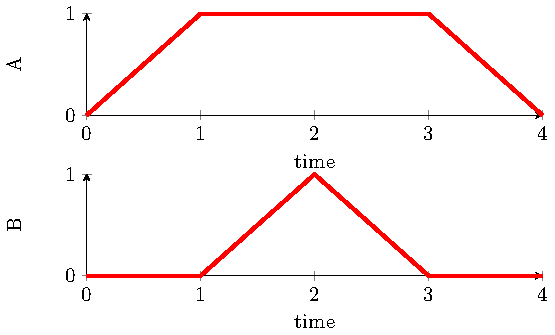
\includegraphics[width=0.8\linewidth]{../figures/AplusBplusBminAmin}
\end{center}
\end{frame}

\begin{frame}[label={sec:orgcbc9d84}]{Implementing the sequence A+B+B-A-, control signal}
\begin{center}
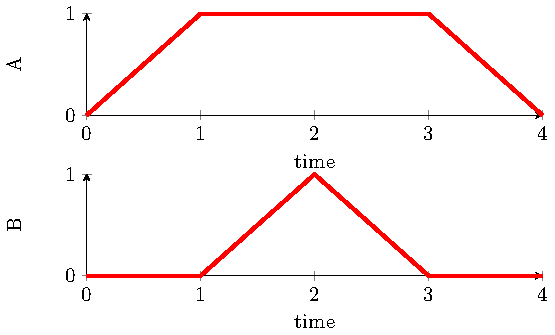
\includegraphics[width=0.3\linewidth]{../figures/AplusBplusBminAmin}
\includegraphics[width=0.68\linewidth]{../figures/logic-control-loop}
\end{center}

\begin{block}{Control signal}
 \[ u = \begin{bmatrix} u_A+ & u_A- & u_B+ & u_B- \end{bmatrix}^T, \]
 with
 \[ u_A+ = \begin{cases} 0 & \text{Solenoid extending A is not activated}\\
                               1&\text{Solenoid extending A is activated}\\
              \end{cases}
   \]
 \[ u_A- = \begin{cases} 0 & \text{Solenoid retracting A is not activated}\\
                               1&\text{Solenoid retracting A is activated}\\
              \end{cases}
   \]
Similar for B.
\end{block}
\end{frame}

\begin{frame}[label={sec:org15b87dc}]{Implementing the sequence A+B+B-A-, state variables}
\begin{center}
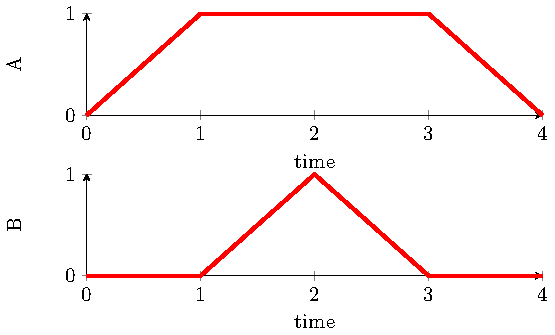
\includegraphics[width=0.3\linewidth]{../figures/AplusBplusBminAmin}
\includegraphics[width=0.68\linewidth]{../figures/logic-control-loop}
\end{center}

\begin{block}{State variables (naive)}
\[ x = \begin{bmatrix} x_A & x_B \end{bmatrix}^T, \]
with
\[ x_{\{A,B\}} = \begin{cases} 0 & \text{Cylinder \{A,B\} retracted}\\
                               1& \text{Cylinder \{A,B\} extended}
                 \end{cases}
   \]
\end{block}
\end{frame}

\begin{frame}[label={sec:org29852ff}]{Implementing the sequence A+B+B-A-, control law}
\begin{center}
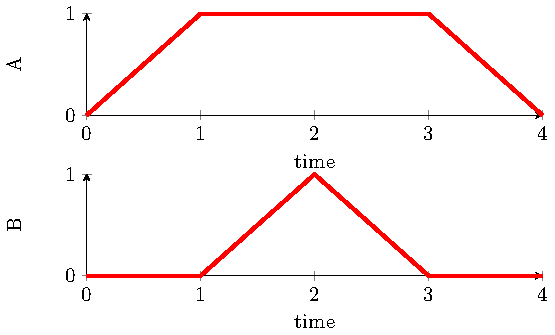
\includegraphics[width=0.3\linewidth]{../figures/AplusBplusBminAmin}
\includegraphics[width=0.68\linewidth]{../figures/logic-control-loop}
\end{center}
\begin{block}{Control law (problematic)}
Ignoring input signal \(u_c\). Movement should be cyclic

\begin{center}
\begin{tabular}{|cc|cccc|}
\hline
\(x_A\) & \(x_B\) & \(u_A+\) & \(u_A-\) & \(u_B+\) & \(u_B-\)\\
\hline
0 & 0 &  &  &  & \\
0 & 1 &  &  &  & \\
1 & 0 &  &  &  & \\
1 & 1 &  &  &  & \\
\hline
\end{tabular}
\end{center}
\end{block}
\end{frame}



\begin{frame}[label={sec:orgfa37bcd}]{Implementing the sequence A+B+B-A-, control law}
\begin{center}
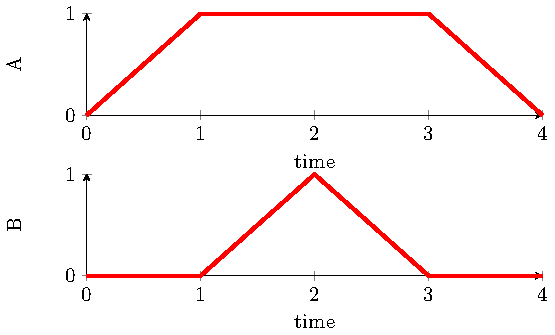
\includegraphics[width=0.3\linewidth]{../figures/AplusBplusBminAmin}
\includegraphics[width=0.68\linewidth]{../figures/logic-control-loop}
\end{center}
\begin{block}{Control law (problematic)}
Ignoring input signal \(u_c\). Movement should be cyclic

\begin{center}
\begin{tabular}{|cc|cccc|}
\hline
\(x_A\) & \(x_B\) & \(u_A+\) & \(u_A-\) & \(u_B+\) & \(u_B-\)\\
\hline
0 & 0 & 1 & 0 & 0 & 0\\
(0) & (1) & 0 & 0 & 0 & 1\\
1 & 0 & 0 & 1 or 0 & 1 or 0 & 0\\
1 & 1 & 0 & 0 & 0 & 1\\
\hline
\end{tabular}
\end{center}
\end{block}
\end{frame}



\begin{frame}[label={sec:org078e432}]{Implementing the sequence A+B+B-A-, state variables}
\begin{columns}
\begin{column}{0.5\columnwidth}
\begin{block}{State variables (better)}
\[ x = \begin{bmatrix} x_A & x_B & x_P\end{bmatrix}^T, \]
with
\[ x_{\{A,B\}} = \begin{cases} 0 & \text{Cylinder \{A,B\} retracted}\\
                               1& \text{Cylinder \{A,B\} extended}
                 \end{cases}
   \]
\[ x_{P} = \begin{cases} 0 & \text{Cheese not yet pressed}\\
                               1& \text{Cheese pressed}
                 \end{cases}
   \]
\end{block}
\end{column}

\begin{column}{0.5\columnwidth}
\begin{block}{State transitions}
\begin{center}
\includegraphics[width=\linewidth]{../figures/AplusBplusBminAmin-withP}
\end{center}
\end{block}
\end{column}
\end{columns}
\end{frame}


\begin{frame}[label={sec:org4339779}]{Implementing the sequence A+B+B-A-, control law}
\begin{columns}
\begin{column}{0.4\columnwidth}
\begin{block}{State transitions}
\begin{center}
\includegraphics[width=\linewidth]{../figures/AplusBplusBminAmin-withP}
\end{center}
\end{block}
\end{column}

\begin{column}{0.6\columnwidth}
\begin{block}{Control law (better)}
\begin{center}
\begin{tabular}{|ccc|cccc|}
\hline
\(x_A\) & \(x_B\) & \(x_P\) & \(u_A+\) & \(u_A-\) & \(u_B+\) & \(u_B-\)\\
\hline
0 & 0 & 0 &  &  &  & \\
1 & 0 & 0 &  &  &  & \\
1 & 0 & 1 &  &  &  & \\
1 & 1 & 1 &  &  &  & \\
\hline
\end{tabular}
\end{center}
\end{block}
\end{column}
\end{columns}
\end{frame}


\begin{frame}[label={sec:org5db74ab}]{Implementing the sequence A+B+B-A-, control law}
\begin{columns}
\begin{column}{0.4\columnwidth}
\begin{block}{State transitions}
\begin{center}
\includegraphics[width=\linewidth]{../figures/AplusBplusBminAmin-withP}
\end{center}
\end{block}
\end{column}

\begin{column}{0.6\columnwidth}
\begin{block}{Control law (better)}
\begin{center}
\begin{tabular}{|ccc|cccc|}
\hline
\(x_A\) & \(x_B\) & \(x_P\) & \(u_A+\) & \(u_A-\) & \(u_B+\) & \(u_B-\)\\
\hline
0 & 0 & 0 & 1 & 0 & 0 & 0\\
1 & 0 & 0 & 0 & 0 & 1 & 0\\
1 & 0 & 1 & 0 & 1 & 0 & 0\\
1 & 1 & 1 & 0 & 0 & 0 & 1\\
\hline
\end{tabular}
\end{center}
\end{block}
\end{column}
\end{columns}
\end{frame}


\begin{frame}[label={sec:orge354360}]{Implementing the sequence A+B+B-A-, control law}
\begin{columns}
\begin{column}{0.4\columnwidth}
\begin{block}{State transitions}
\begin{center}
\includegraphics[width=\linewidth]{../figures/AplusBplusBminAmin-withP}
\end{center}
\end{block}
\end{column}

\begin{column}{0.6\columnwidth}
\begin{block}{Control law (better)}
\begin{center}
\begin{tabular}{|ccc|cccc|}
\hline
\(x_A\) & \(x_B\) & \(x_P\) & \(u_A+\) & \(u_A-\) & \(u_B+\) & \(u_B-\)\\
\hline
0 & 0 & 0 & 1 & 0 & 0 & 0\\
1 & 0 & 0 & 0 & 0 & 1 & 0\\
1 & 0 & 1 & 0 & 1 & 0 & 0\\
1 & 1 & 1 & 0 & 0 & 0 & 1\\
\hline
\end{tabular}
\end{center}

\begin{align*}
  u_A+ &= \not{x_A}\\
  u_A- &= x_A\not{x_B}x_P\\
  u_B+ &= x_A\not{x_B}\not{x_P}\\
  u_B- &= x_B
\end{align*}
\end{block}
\end{column}
\end{columns}
\end{frame}


\begin{frame}[label={sec:orge4b7ee1}]{Implementing the sequence A+B+B-A-, latching circuit for \(x_P\)}
\begin{columns}
\begin{column}{0.3\columnwidth}
\begin{center}
\includegraphics[width=\linewidth]{../figures/AplusBplusBminAmin-withP}
\end{center}
\end{column}

\begin{column}{0.7\columnwidth}
\begin{LaTeX}
\begin{center}
         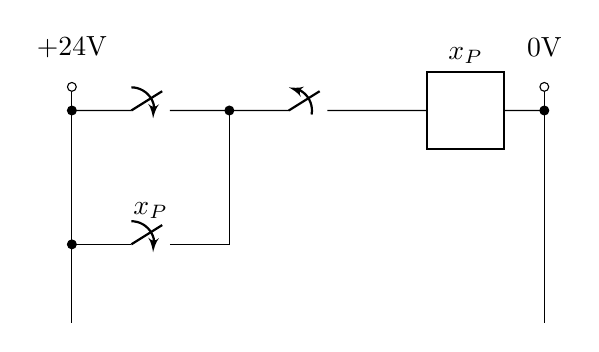
\begin{tikzpicture}
           \node at (0,0.5) {+24V};
           \node at (6,0.5) {0V};
           \draw (0,0) to[short, o-]  (0,-3);
           \draw (6,0) to[short, o-](6,-3);
           \draw (0,-0.3) to[switch, *-, ] (2,-0.3) to[ opening switch,  ] (4,-0.3) to[short] (4,-0.3) to[twoport, label=$x_P$, -*] (6,-0.3);
           \draw (0,-2) to[switch, *-, label=$x_P$] (2,-2)  to[short,-*] (2,-0.3);
         \end{tikzpicture}
\end{center}
\end{LaTeX}

Implement the circuit!
\end{column}
\end{columns}
\end{frame}

\begin{frame}[label={sec:orga7db220}]{For the report}
\begin{itemize}
\item Truth table for the control law
\item Control law as boolean expression
\item Circuit diagram for the controller
\item Screen shot and short video showing working solution in FluidSim
\item Short video showing working solution in hardware
\end{itemize}
\end{frame}
\end{document}